\documentclass[10pt,a4paper]{article}
\usepackage[utf8]{inputenc}
\usepackage[spanish]{babel}
\usepackage{a4wide}
\usepackage[sinEntregas]{caratula}
\usepackage{ulem}
\usepackage{marginnote}
\usepackage{fancyhdr}
\usepackage{lastpage}
\usepackage{float}
\usepackage{tikz}
\usepackage{mattens}

\pagestyle{fancy}
\thispagestyle{fancy}
\addtolength{\headheight}{1pt}
\lhead{Bases de Datos}
\rhead{TP2}
\cfoot{\thepage /\pageref{LastPage}}
\renewcommand{\thesubsubsection}{\thesubsection.\alph{subsubsection}}

\title{Bases de Datos - TP 2}
\author{Bases de Datos, DC, UBA.}

\begin{document}

\fecha{Bases de Datos}

\materia{Informe Técnico}
%\submateria{Trabajo Pr\'actico Nº1}
\titulo{Web Semántica}

\integrante{Allocati, Federico}{682/11}{fede.allocati@gmail.com}
\integrante{Izcovich, Sabrina}{550/11}{sizcovich@gmail.com}
\integrante{Pernigotti, Santiago}{870/11}{spernigotti@hotmail.com}
\integrante{Romano, Germán}{786/11}{romano.german@live.com.ar}

\maketitle

\tableofcontents

\newpage

\section{Introducción}

El siguiente informe consiste en un análisis técnico enfocado en la \textit{Web Semántica}. Para la realización del mismo, basamos nuestra investigación en la tesis\footnote{http://dc.uba.ar/inv/tesis/licenciatura/2013/bursztyn.pdf} presentada por \textit{Damián A. Bursztyn} en el año 2013 sobre \textbf{Optimización de consultas RDF reformuladas} y en el artículo \textbf{Introduction to the Special Issue on Semantic Web Data Management} escrito por \textit{Roberto De Virgilio} en 2011.

En lo que sigue, explicaremos los conceptos de Web Semántica y sus problemáticas, de su formato de representación \textit{RDF} y de los mecanismos que ayudan a convertir la Web en una infraestructura global en la que es posible compartir, y reutilizar datos y documentos entre diferentes tipos de usuarios.

\section{Web Semántica}
La Web Semántica consiste en una Web Extendida dotada de mayor significado gracias a los metadatos que acompañan a los datos que circulan. Su utilidad principal es encontrar soluciones a problemas habituales en la búsqueda de información gracias a la utilización de una infraestructura común mediante la que se procesa y transfiere información de una manera sencilla. Esta Web extendida y basada en el \textit{significado}, se apoya en lenguajes universales que resuelven los problemas ocasionados por una Web carente de semántica en la que, en ocasiones, el acceso a la información se convierte en una tarea difícil.\\

Es menester aclarar algunos conceptos que se utilizarán a lo largo del trabajo:
\begin{itemize}
\item Las tecnologías de \textbf{Web Semántica} son gobernadas por el \textbf{W3C} (\textit{World Wide Web Consortium}).
\item Los estándares más utilizados son \textbf{RDF} (\textit{Framework de Descripción de Recursos}) y \textbf{SPARQL} (\textit{Lenguaje de Queries RDF}).
\item \textbf{RDF} se usa para el almacenado y representación de datos y \textbf{SPARQL} es el lenguaje de consulta que devuelve los datos de un almacenamiento \textbf{RDF}.\\
Luego, un set de datos \textbf{RDF} consiste en datos explícitos e implícitos presentes en la base de datos, dados por restricciones semánticas que deben cumplir. Dichos datos son obtenidos por un proceso que considera las restricciones para inferir todas las posibles consecuencias de la base de datos existente.
\end{itemize}

\section{RDF y RDF Schema}
RDF provee un lenguaje simple que permite describir metadatos sobre recursos web en forma de triplas $<s$ $p$ $o>$. Una tripla establece que el valor de la propiedad $p$ para el sujeto $s$ es el objeto $o$. El sujeto y la propiedad son URIs dirigidas a recursos web, mientras que el objeto puede ser tanto una URI como un valor constante. 
\\
Una característica importante de RDF son los $blank nodes$, ya que permiten representar constantes o URIs desconocidas. En una tripla RDF un $blank node$ es un sujeto u objeto que no identifica ni una URI ni un valor. La notación usada para referirnos a ellos es la de $\_ :b$
\\
$s$ $\tau$ $o$ declara que el sujeto $s$ pertenece a la clase $o$.
  
\begin{figure}[H]
\begin{center}
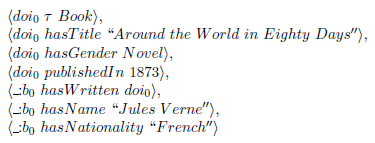
\includegraphics[width=260pt]{imgs/ejemplo_rdf}
\caption{Ejemplo de RDF}
\end{center}
\end{figure}

En el ejemplo previo se describe el hecho de que ``Around the World in Eighty Days'' es un libro, del género novela, que fue publicado en 1873 y escrito por Julio Verne.

Una alternativa a la representación dada, es representar las triplas en forma de grafo dirigido, donde los nodos son sujetos u objetos etiquetados con sus valores y las aristas son las propiedades.
\\
\begin{figure}[H]
\begin{center}
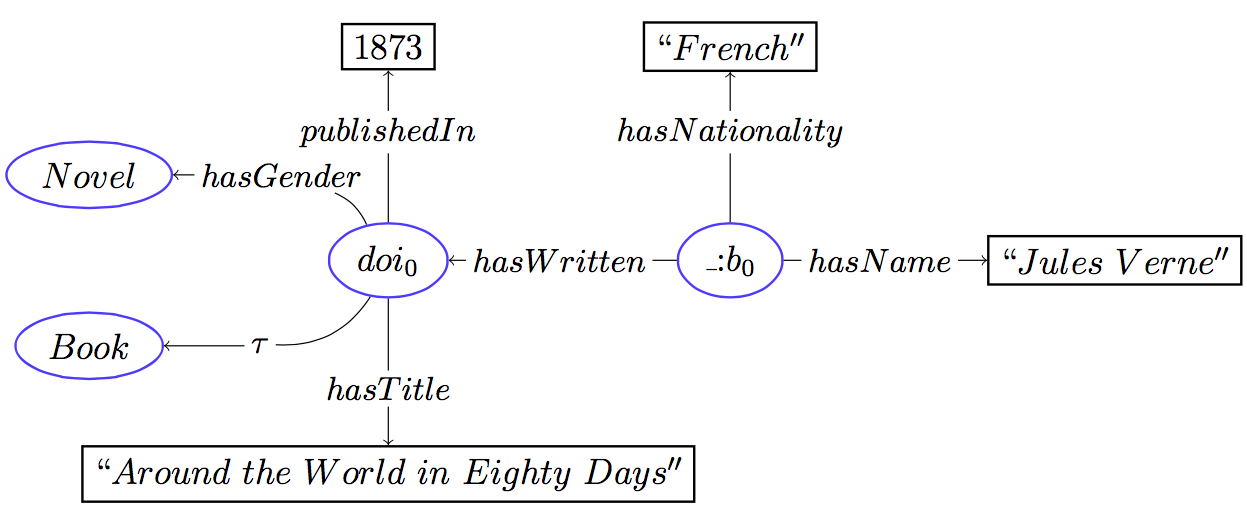
\includegraphics[width=400pt]{imgs/ejemplo_rdfgrafo}
\caption{Ejemplo RDF representado como grafo}
\end{center}
\end{figure}

RDFS (RDF squema) es una extensión de RDF que mejora el poder descriptivo de un $dataset$ RDF a través de la declaración de restricciones. Un RDFS especifica restricciones de los individuos (clases) y las relaciones (propiedades) usadas en las triplas RDF, habilitando \textit{encolamiento}\footnote{http://www.w3.org/TR/rdf11-mt/\#rdf-entailment} (una de las características más importantes de la Web Semántica). 

En el ejemplo anterior, se presenta un $dataset$ dentro del que se presenta que \textit{Julio Verne} ha escrito el libro ``Around the World in Eighty Days''. Como un RDFS puede establecer que todos los que escriben libros son escritores, el hecho de que \textit{Julio Verne} sea un escritor está implícito en el $dataset$.
\newpage
En la siguiente tabla se pueden observar posibles tipos de restricciones. $Domain$\footnote{Dominio} y $range$\footnote{rango} denotan, respectivamente, el primer y el segundo atributo de cada propiedad.

\begin{figure}[h]
\begin{center}
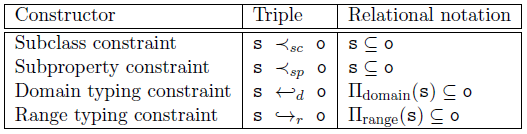
\includegraphics[width=250pt]{imgs/constraints}
\caption{Restricciones en RDFS}
\end{center}
\end{figure}

\section{Web Semántica y Manejo de Datos}
El exponencial crecimiento de los datos en la web deja en claro la necesidad de complementar el estudio de la Web Semántica con dos disciplinas bien desarrolladas: modelado conceptual y manejo de datos. 
\\
El Modelado Conceptual se encarga del desarrollo de técnicas avanzadas y herramientas que permiten la representación precisa y el razonamiento de artefactos que modelan objetos e información del mundo real. El Manejo de Datos, en cambio, se encarga del desarrollo de técnicas para el eficiente almacenamiento, consultas, recuperación y manejo de grandes volúmenes de información de diferente naturaleza, es decir, datos relacionales, documentos XML, blogs, etc.
\\
A continuación se presentan contribuciones que abarcan las tres áreas; Web Semántica, Modelado Conceptual y Manejo de Datos.
\\\\
\textbf{Quality-aware} propone algunas estrategias para diseñar funciones de similitud que capturan el grado de libertad para la equivalencia de dos entidades dadas. El método se basa en la combinación de múltiples evidencias, con la ayuda de calidad estimada de valores individuales similares y con la particular atención a la perdida de información, que es común en el contexto de la web. 
\\\\
\textbf{Structured Data Clouding across Multiple Webs} introduce la noción de inCloud, una colección de recursos web relacionados construidos para una entidad objetivo de interés mediante la distinción, también en una forma visual, de que tan prominente es cada recurso web recibido con respecto a la entidad dada
\\\\
\textbf{Ontological Query Answering under Expressive Entity-Relationship Shemata} contribuye a reducir la brecha entre modelos conceptuales y razonamiento semántico, abordando el problema de respuestas a consultas conjuntivas bajo restricciones representadas por esquemas expresados en ER+, una extensión del modelo entidad-relación.
\\\\
\textbf{PEST: Fast Approximate Keyword Search in Semantic Data using Eigenvector-based Term Propagation} presenta un novedoso enfoque a las consultas aproximadas de datos sobre grafos-estructurados RDF que propagan términos ponderados entre ítems de datos que son conectados en la estructura de datos.
\\\\
\textbf{An Ontology-Based Retrieval System Using Semantic Indexing} introduce un sistema para ontologías basadas en extracción de información.
\\\\
\textbf{A step forward is taken in PoweR-Gen: A Power-law Based Generator of RDFS Schemas} presenta el primer generador de esquemas RDF, teniendo en cuenta las características exhibidas por los esquemas reales SW.

\section{Problemas de la Web Semántica}
En el último tiempo, el uso de Web Semántica creció enormemente e impulsó la necesidad de emplear técnicas eficientes y escalables para responder a las consultas RDF sobre una gran cantidad de datos heterogéneos. Una posible solución a este problema consiste en traducir las consultas RDF en consultas SQL para ejecutarlas en los sistemas de gestión de bases de datos relacionales (RDBMS). Sin embargo, las bases de datos para Web Semántica complican a las tecnologías clásicas de gestión de datos que no tienen en cuenta los datos implícitos durante la evaluación de consultas. Una solución a esto es reformular la consulta entrante para luego traducirla en una consulta SQL que, al ser evaluada por el RDBMS, devuelve las respuestas completas. El problema que esta solución presenta es de rendimiento debido a la longitud sintáctica de las consultas SQL que resultan de reformulación. Los RDBMSs no son capaces de optimizar eficientemente estas consultas, por lo que en algunos casos fallan o registran tiempos elevados de evaluación.

\section{SPARQL}
Es el estándar W3C para consultas RDF. En otras palabras, es un lenguaje de consultas semánticas para bases de datos, habilitado para devolver y manipular datos guardados en el formato RDF. El mismo permite hacer búsquedas sobre los recursos de la Web Semántica utilizando distintas fuentes datos.

\section{Basic Graph Pattern}
Las consultas BGP son un subconjunto del lenguaje de consultas SPARQL W3C para RDF. El mismo se corresponde con la clase de familias de consultas conjuntivas de las bases de datos relacionales. Además, las BGP conforman las consultas SPARQL más utilizadas en el mundo real.
Principalmente, están compuestas por un conjunto de variables distinguidas, la cabeza y el conjunto de patrones de tripla (los BGP).

\subsection{Ejemplo}
\begin{figure}[H]
        \setbox0\hbox{%
                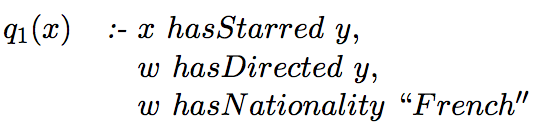
\includegraphics[width=.45\textwidth]{./imgs/ejemploBGP-02.png}%
        }%
        \setbox2\hbox{%
                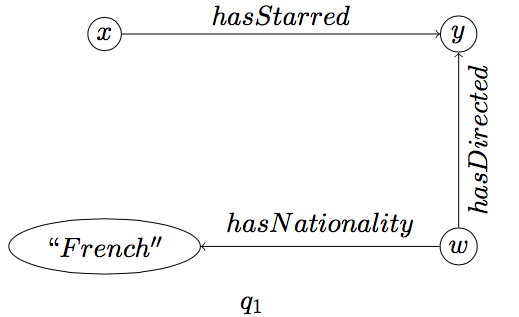
\includegraphics[width=.45\textwidth]{./imgs/ejemploBGP-02_grafico.png}%
        }%
        \ifdim\ht0>\ht2
                \setbox0\hbox{%
                        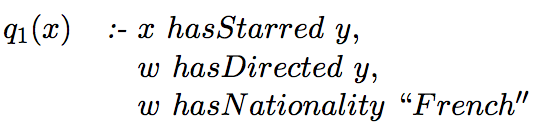
\includegraphics[height=\ht2]{./imgs/ejemploBGP-02.png}%
                }%
        \else
                \setbox2\hbox{%
                        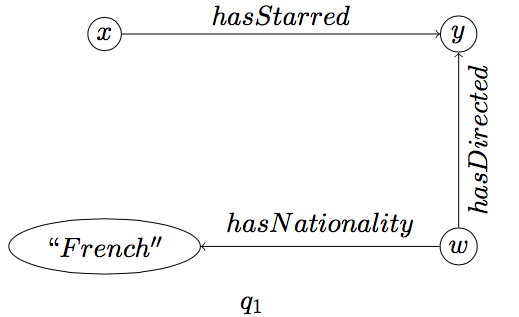
\includegraphics[height=\ht2]{./imgs/ejemploBGP-02_grafico.png}%
                }%
        \fi
        \noindent
        \parbox{.45\textwidth}{%
                \centering
                \unhbox0
                \caption{Consulta RDF}
                \label{fg:methods}
        }%
        \hfil
        \parbox{.45\textwidth}{%
                \centering
                \unhbox2
                \caption{Grafo RDF}
                \label{fg:method_detail}
        }%
\end{figure}
\vspace*{0.3cm}
Consulta que devuelve los actores que trabajaron en una película dirigida por un francés.

\section{SPARQL y BGP}

\begin{figure}[H] %[h] Aqui [b] para button [t] para top
\begin{center}
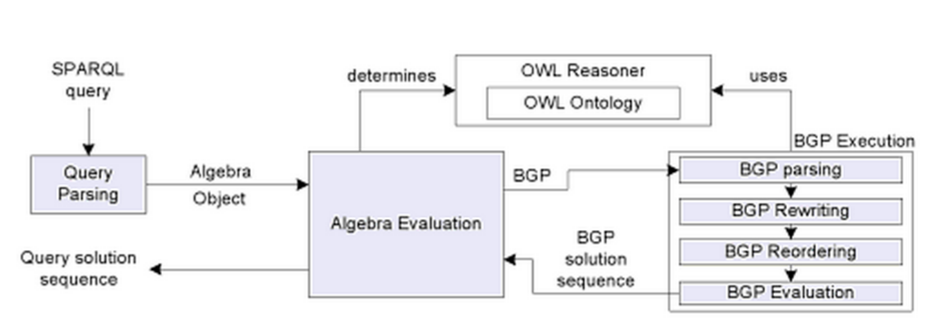
\includegraphics[width=400pt]{./imgs/conceptos.png}
\caption{Relación entre conceptos.}
\end{center}
\end{figure}

\section{RDF y RDBMS}
Una alternativa frente a las tradicionales tablas de datos relacionales que incluyen valores NULL en ellas, son las tablas-V. Estas permiten el uso de variables en sus filas, la cual es una característica importante porque posibilita el uso de juntas para valores desconocidos, dado que es posible utilizar la misma variable en diferentes filas.
\\\\
Utilizando la evaluación del sistema de gestión de base de datos relacionales (RDBMS), podemos obtener el conjunto de respuestas de consultas BGP de la siguiente forma:

Dado un conjunto de datos $D$, podemos almacenarlo todo en una tabla-V de la forma Triples(s,p,o), guardando los triples de $D$ dentro de la tabla como filas, y además convirtiendo los nodos blancos en variables. Entonces, dado una consulta BGP de la forma $q(x) : s_{1} p_{1} o_{1}, ..., s_{n} p_{n} o_{n}$, se puede reescribir como una consulta conjuntiva para la evaluación del RDBMS del siguiente modo:
\\
$q(x): \wedge ^n _{i = 1} Triples(s_{i}, p_{i}, o_{i})$
\\\\
Mediante dos técnicas establecidas para el manejo de vinculación RDF, llamadas saturación y reformulación, podemos calcular la respuesta de la consulta $q$ en $D$.
\\\\
\textbf{Saturación}: Se evalúa la consulta $q(x): \wedge ^n _{i = 1} Triples(s_{i}, p_{i}, o_{i})$ en la tabla Triples que contenga la clausura de $D$ (todos los datos implícitos se encuentran dentro de la tabla). Esta técnica calcula la clausura del conjunto de datos usando las reglas de vinculación. Sus desventajas son que para calcular el conjunto de datos completo requiere tiempo de cómputo y espacio de almacenamiento, y debe ser recalculado por cada actualización realizada.
\\
\begin{figure}[h]
\begin{center}
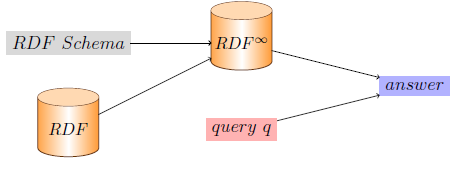
\includegraphics[width=270pt]{imgs/saturacion}
\caption{Visión general del proceso de respuesta de una consulta basada en saturación.}
\end{center}
\end{figure}
\\
\textbf{Reformulacion}: Se evalúa $q'(x): \wedge ^n _{i = 1} Triples(s_{i}, p_{i}, o_{i})$ en la tabla Triples que contenga a $D$, donde $q'$ es la reformulación de la consulta $q$. La reformulación se realiza utilizando reglas de vinculación inmediatas, de manera tal que la consulta $q'$ sobre $D$ sea equivalente a $q$ sobre la clausura de $D$. La principal ventaja de este método es que no se ve afectado por las actualizaciones, ya que no es necesario recalcular la clausura del conjunto de datos. 

\begin{figure}[H]
\begin{center}
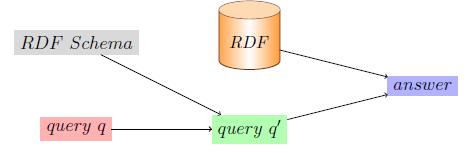
\includegraphics[width=270pt]{imgs/reformulacion}
\caption{Visión general del proceso de respuesta de una consulta basada en reformulación.}
\end{center}
\end{figure}


\section{Reformulación de Consultas}

Dada una query q y un \textit{dataset} D, queremos reformular q con respecto al esquema D en otra query q$'$ tal que la evaluación de q$'$ contra los datos de D (es decir, q$'$(D$_{data}$)) sea el conjunto respuesta completo de q contra D (o sea, q(D$^{\infty}$)).

\subsection{Consultas Parcialmente Instanciadas}

Sea $q(\bS{x}) :- t_{1},...,t_{n}$ una query y $\sigma$ un mapeo de un subconjunto de variables y \textit{blank nodes} de q a algunos valores (constantes, URIs o \textit{blank nodes}).\\

Una \textbf{consulta parcialmente instanciada} con respecto a q, notada $q_{\sigma}$, es una query $q_{\sigma}(\bS{x}_{\sigma}) :- (t_{1},...,t_{n})_{\sigma}$ donde el mapeo $\sigma$ fue aplicado tanto en las variables de la cabeza como en las variables del cuerpo de q. En el caso $\sigma = \emptyset$, vale $q_{\sigma} = q$.\\

Dada una consulta parcialmente instanciada $q_{\sigma}(\bS{x}_{\sigma}) :- (t_{1},...,t_{n})_{\sigma}$ cuyo conjunto de variables y \textit{blank nodes} es VarBl($q_{\sigma}$) y un \textit{dataset} D cuyo conjunto de valores es Val(D), la evaluación de $q_{\sigma}$ contra D es:\\
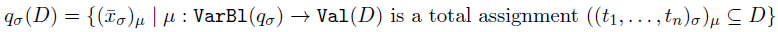
\includegraphics[scale=0.45]{imgs/01.png}\\

El conjunto respuesta completo de $q_{\sigma}$ contra D es $q_{\sigma}(D^{\infty})$.

\subsection{Reglas de Reformulación}

A continuación se muestran las 13 reglas de reformulación, cada una definiendo una transformación de la forma $\frac{input}{output}$, para una consulta parcialmente instanciada $q_{\sigma}$ con respecto a un \textit{dataset} D:

\begin{center}
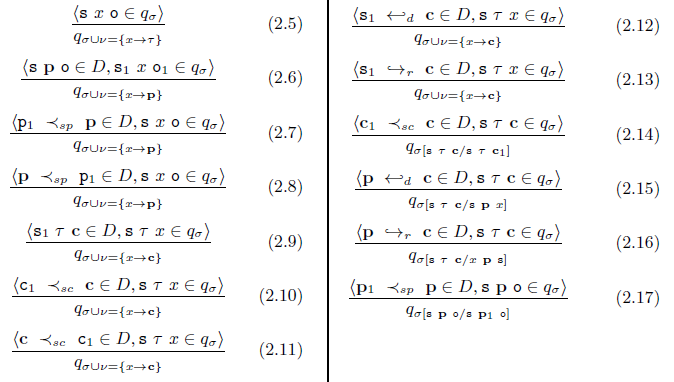
\includegraphics[scale=0.8]{imgs/02.png}
\end{center}

Se pueden distinguir dos grupos de reglas:
\begin{itemize}

\item Las reglas 2.5 hasta 2.13 reformulan la query bindeando una de las variables de la query a la propiedad RDF $\tau$ ó a una clase o propiedad definida en el \textit{dataset}.

\item Las reglas de 2.14 a 2.17 alteran las queries reemplazando una de sus triplas por otra, mediante el uso de esquemas.

\end{itemize}

\subsection{Resolución de Consultas Basada en Reformulación}

La resolución de consultas basada en reformulación reformula una query q con respecto a las restricciones definidas en el esquema RDF del \textit{dataset} D en una query q$'$ tal que $q'(D_{data}) = q(D^{\infty})$.\\

La técnica de reformulación de consultas mostrada en las subsecciones anteriores no cumple con lo anterior, a causa de la indistinguibilidad de los \textit{blank nodes}.\\

Para solucionar esto, se define lo siguiente:

\begin{itemize}

\item La \textbf{evaluación no estándar} de una query parcialmente instanciada $q_{\sigma}$ contra un \textit{dataset} D, siendo Var($q_{\sigma}$) el conjunto de variables de q y Val(D) el conjunto de valores de D, se define como:\\
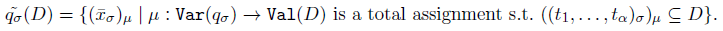
\includegraphics[scale=0.5]{imgs/03.png}\\
Observación: los \textit{blank nodes} quedan intactos.

\item La siguiente \textbf{propiedad} relaciona evaluación y conjunto respuesta estándar y no estándar.\\
Sea D \textit{database} y $q_{\sigma}$ una query parcialmente instanciada contra D, vale:

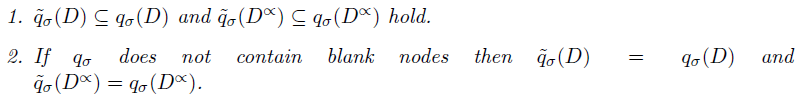
\includegraphics[scale=0.5]{imgs/04.png}

\item \textbf{Teorema}: (nueva técnica para resolver consultas basada en reformulación) Sea q una query BGP sin \textit{blank nodes} y D un \textit{dataset} cuyo esquema es S, vale:

\begin{center}
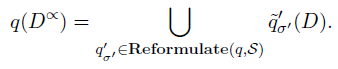
\includegraphics[scale=0.55]{imgs/05.png}
\end{center}

\end{itemize}

\subsection{Algoritmo de Reformulación}

El algoritmo de reformulación toma la query original q y las reglas de reformulación detallas anteriormente para generar nuevas queries mediante la aplicación de dichas reglas a los átomos de q. Se procede iterativamente sobre el resultado obtenido hasta que no se obtengan nuevas queries. Finalmente, se devuelve la unión de las nuevas queries generadas y la query original.\\

En cada iteración del algoritmo mostrado a continuación se matchean los átomos de la query con el input de cada regla; de haber coincidencia, se aplica dicha regla.\\

Este algoritmo termina, es correcto y completo. La complejidad de la reformulación de queries es polinomial en el tamaño del esquema y exponencial en el tamaño de la query. La resolución de la consulta contra un \textit{dataset} D está en LogSpace en el tamaño de D y es exponencial en el tamaño de la query.\\

\vspace{100 mm}

\begin{center}
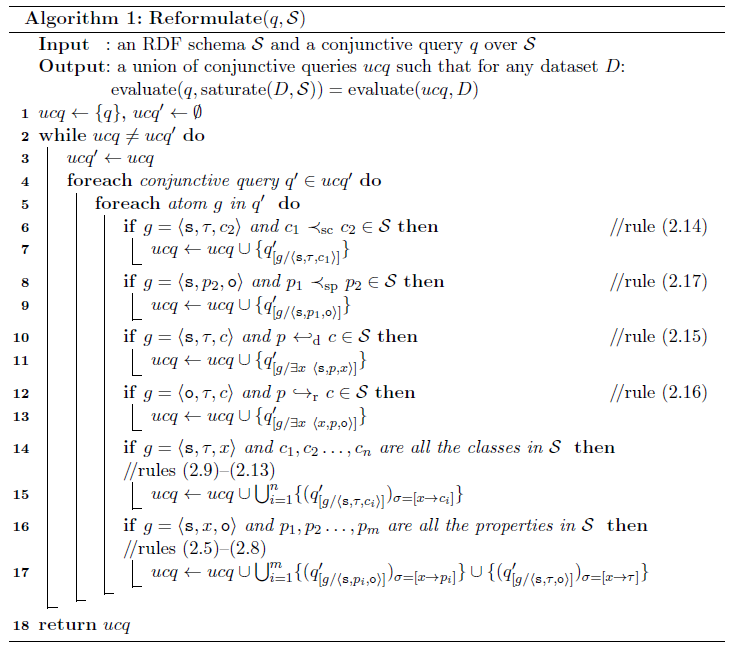
\includegraphics[scale=0.55]{imgs/06.png}
\end{center}

\section{Referencias}

\begin{itemize}
\item The World Wide Web Consortium (W3C). http://www.w3c.es/Divulgacion/GuiasBreves/WebSemantica
\item http://jplu.developpez.com/tutoriels/web-semantique/introduction/
\end{itemize}

\end{document}